\newpage
\section{\textit{Aleksander Pyrdek}}
\label{sec:apyrdek}


\begin{figure}[H]
    \centering
    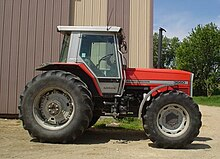
\includegraphics[width=0.8\textwidth]{pictures/traktor.jpg} 
    \caption{To zdjecie przedstawia traktor.}
    \label{fig:traktor}
\end{figure}

Wyrażenie matematyczne: \[a^2 = a*a\]

\begin{table}[H]
    \centering
    \begin{table}[H]
\centering
\begin{tabular}{|l|l|l|l|l}
\cline{1-4}
Jeden & Dwa & Trzy & Cztery &  \\ \cline{1-4}
1     & 2   & 3    & 4      &  \\ \cline{1-4}
2     & 3   & 4    & 5      &  \\ \cline{1-4}
3     & 4   & 5    & 6      &  \\ \cline{1-4}
\end{tabular}
\end{table}
\end{table}

\textbf{To jest lista 3 najpopularniejszych traktorów:}

\begin{enumerate}
  \item John Deere 8R Series
  \item Case IH Magnum Series
  \item New Holland T7 Series
\end{enumerate}

\textit{To jest lista 3 najpopularniejszych traktorów:}

\begin{itemize}
  \item[--] Pierwszy element
  \item[--] Drugi element
  \item[--] Trzeci element
\end{itemize}

\textbf{Lorem Ipsum\\}

Lorem ipsum dolor sit amet, consectetur adipiscing elit, sed do eiusmod tempor incididunt ut labore et dolore magna aliqua. Ut enim ad minim veniam, quis nostrud exercitation ullamco laboris nisi ut aliquip ex ea commodo consequat. Duis aute irure dolor in reprehenderit in voluptate velit esse cillum dolore eu fugiat nulla pariatur. Excepteur sint occaecat cupidatat non proident, sunt in culpa qui officia deserunt mollit anim id est laborum.

A lacus vestibulum sed arcu non odio. Cras semper auctor neque vitae tempus quam. Mattis ullamcorper velit sed ullamcorper morbi. Tellus rutrum tellus pellentesque eu tincidunt tortor aliquam. Pellentesque habitant morbi tristique senectus et netus et. Fermentum iaculis eu non diam phasellus vestibulum lorem. Mauris augue neque gravida in fermentum et sollicitudin ac. Posuere morbi leo urna molestie at elementum eu facilisis. Proin libero nunc consequat interdum. Eget mauris pharetra et ultrices neque. Orci dapibus ultrices in iaculis nunc. Lorem mollis aliquam ut porttitor. Augue mauris augue neque gravida in fermentum et sollicitudin. Ipsum consequat nisl vel pretium. Mauris sit amet massa vitae tortor condimentum. Ultricies mi eget mauris pharetra et ultrices neque ornare aenean.